\documentclass[a4paper,12pt,oneside,openany,table,xcdraw]{article}

\usepackage{setspace}
\usepackage{multirow}
\usepackage{hyperref}
\usepackage{caption}
\usepackage{indentfirst}

\usepackage[brazilian]{babel}
\usepackage[utf8x]{inputenc}
\usepackage{amsmath, graphicx, mathptmx, enumerate}
\usepackage{float, verbatim}
\usepackage[colorinlistoftodos]{todonotes}
\usepackage{makeidx} % Para o sumário
\usepackage{geometry}

\geometry{a4paper, hmargin={3cm, 3cm}, vmargin={3cm, 2cm} }
\setlength{\parindent}{1.0cm}

\begin{document}
\newcommand{\thedepartment}{Faculdade de Engenharia Elétrica}
\newcommand{\thecourse}{FEELT}
\newcommand{\thetitle}{TENSÕES, CORRENTE E POTÊNCIAS EM CIRCUITO SÉRIE, FATOR DE POTÊNCIA E CORRENTE ALTERNADA SENOIDAL - USO DE MEDIDORES ANALÓGICOS E DIGITAIS}
\newcommand{\thetype}{Relatório da Disciplina de Circuitos Elétricos II}
\newcommand{\theproftitle}{Bacharel em Engenharia Elétrica}
\newcommand{\thestudent}{Lesly Viviane Montúfar Berrios\\
\centering11811ETE001}
\newcommand{\theadvisor}{Prof. Wellington Maycon Santos Bernardes}
\newcommand{\thecity}{Uberlândia}

\thispagestyle{empty}\newcommand*{\themonth}{\ifthenelse{\the\month < 2}{Janeiro }
                  {\ifthenelse{\the\month < 3}{Fevereiro }
                  {\ifthenelse{\the\month < 4}{Março }
                  {\ifthenelse{\the\month < 5}{Abril }
                  {\ifthenelse{\the\month < 6}{Maio }
                  {\ifthenelse{\the\month < 7}{Junho }
                  {\ifthenelse{\the\month < 8}{Julho }
                  {\ifthenelse{\the\month < 9}{Agosto }
                  {\ifthenelse{\the\month < 10}{Setembro }
                  {\ifthenelse{\the\month < 11}{Outubro }
                  {\ifthenelse{\the\month < 12}{Novembro }{Dezembro }}}}}}}}}}}}
                  
\begin{titlepage}
\begin{center}

	\vspace{-0.5cm}

  \begin{figure}[hbt!]
		\begin{center}
		   
\includegraphics[width=2.8cm]{ufu-logo.png}
		\end{center}
	\end{figure}
 	%\vspace{-4cm}

%\begin{doublespacing}

  \Large{\textbf{Universidade Federal de Uberlândia}}\\
  \large{\thedepartment}\\
  \large{\thecourse}\\


\vspace{5.8cm}
  \par
  \large\textbf{\thetitle}
\vspace{5.8cm} 

%\end{doublespacing}
  \par
  \thetype\\
  por\\
  %\hspace{2cm}\large{}\\

\vspace{0.8cm}
\par
  \normalsize{\thestudent}\\ [2cm]
  \theadvisor

\par\vfill
  \thecity, \themonth / \the\year

\end{center}

\end{titlepage}

%% Comeca o documento !

\onehalfspacing
\tableofcontents % sumário
\newpage

\section{Objetivos} % 2,5%
Montar um circuito série \emph{RLC}, energizá-lo com tensão alternada senoidal, realizar medições usando
equipamentos analógicos e digitais, efetuar desenvolvimentos teóricos e cálculos numéricos confrontando os
resultados teóricos com aqueles obtidos experimentalmente.

\section{Introdução teórica} % 5%




\section{Preparação}
\subsection{Materiais e ferramentas} % 2,5%
\begin{enumerate}[1 - ]
\item \emph{Fonte}\\
Alimentará todo o circuito.

\item \emph{Variador de tensão (Varivolt)}\\
O equipamento permitirá obter o valor desejado de corrente a partir da regulagem correta da tensão fornecida pela fonte. Também chamado de autotransformador.

\item \emph{Medidor eletrônico KRON Mult K}\\
Possibilita encontrar a medição da potência
real (P) - vatímetro, reativa (Q) e aparente (S) do circuito. Ele também possui função de cofasímetro, instrumento elétrico que mede o fator de potência (fp, $cos\theta$) ou o ângulo da impedância $\theta$ do circuito, para um circuito com a impedância $Z = Z\angle \theta$.

\item \emph{Conectores}\\
Foram utilizadas pontas de provas para a verificação das grandezas nos multímetros e pontas de prova específicas para multímetro. Para as conexões no circuito foi utilizado majoritariamente cabos banana-banana.

\item \emph{Multímetro}\\
Utilizado para medir a resistência R, capacitância C e gradezas do conjunto L e $R_L$ especificados no experimento.

\item \emph{Amperímetro analógico AC}\\
Instrumento de maior precisão.

\item \emph{Voltímetro analógico AC}\\
Instrumento de maior precisão.

\item \emph{Osciloscópio}\\
Utilizado obter informações da forma de onda ($V_{pp}$,$V_{max}$, $V_{rms}$).

\item \emph{Reostato R}\\
Reostato com potência nominal de aproximadamente 1kW.

\item \emph{Capacitor C}\\
Reostato com potência nominal de aproximadamente 1kW.

\item \emph{Bobina B}\\
O valor medido da indutância da bobina B (reator para lâmpada vapor de sódio) realizada
recentemente (Agosto/2019) é de 160 mH e resistência interna de 3,8 ohms.

\end{enumerate}

\subsection{Montagem} % 2,5%

\begin{enumerate}[1)]
\item \emph{Montando o circuito}\\
Realize a montagem informada na Figura \ref{fig1}, com os parâmetros R, C, L, RL, V e f (preenchendo as
Tabelas 1 e 2). 

\begin{figure}[H]
\centering
\captionsetup{font=scriptsize}
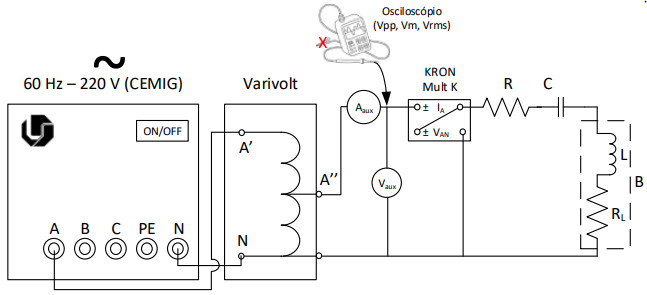
\includegraphics[width=14.5cm]{fig1}
\caption{Montagem experimental.}
\label{fig1}
\end{figure}

\end{enumerate}

\section{Análise sobre segurança} % 2,5%
Os óculos de segurança são Equipamentos de Proteção Individual (EPIs) e são utilizados para a proteção da área ao redor dos olhos contra qualquer tipo de detrito estranho, que possa causar irritação ou ferimentos. Também protegem contra faíscas, respingos de produtos químicos, detritos, poeira, radiação e etc \cite{safe}.
É importante a utilização desse equipamento durante os experimentos a fim de evitar qualquer dano, além de preparar o profissional para o manejo correto e seguro de qualquer equipamento.
Além disso, foi de extrema importância a presença do professor ou técnico na verificação da montagem do circuito antes de energizá-lo. Assim, reduziu-se riscos de curtos-circuitos ou sobrecarga na rede.

\section{Cálculos, análise dos resultados e questões} % (quando houver) (70%)

\begin{enumerate}[1 - ]
\item Complete a Tabela \ref{tab1} com os dados do Caso A, sendo $V_{ef}=100V$ e $R=100\Omega$ (teórico).

\begin{table}[h]
\centering
\def\arraystretch{1.35}
\captionsetup{font=scriptsize}
\captionof{table}{Parâmetros reais da montagem do primeiro caso.} \label{tab1}
\begin{tabular}{|c|c|c|c|c|c|}
\hline
$R [\Omega]$ & $V (V)$ & $L [mH]$ & $R_L [\Omega]$ & $V [volts]$ & $f [Hz]$ \\ \hline
       100      &         &          &                &      99,4       &     59,95     \\ \hline
\end{tabular}
\end{table}

\item Complete a Tabela \ref{tab2} com os dados do Caso B, sendo $V_{ef}=50V$ e $R=20\Omega$ (teórico).

\begin{table}[h]
\centering
\def\arraystretch{1.35}
\captionsetup{font=scriptsize}
\captionof{table}{Parâmetros reais da montagem do segundo caso.} \label{tab2}
\begin{tabular}{|c|c|c|l|l|l|}
\hline
$R [\Omega]$ & $V (V)$ & $L [mH]$ & $R_L [\Omega]$ & $V [volts]$ & $f [Hz]$ \\ \hline
       20      &         &          &                &       49,39      &     60,00     \\ \hline
\end{tabular}
\end{table}

\item Ajuste a tensão de saída do autotransformador (varivolt) de maneira a obter a tensão solicitada para o voltímetro e anote os valores medidos na Tabela \ref{tab3} (para ambos os casos, A e B).
\begin{table}[H]
\centering
\def\arraystretch{1.35}
\captionsetup{font=scriptsize}
\captionof{table}{Erro percentual das duas montagens.} \label{tab3}

\resizebox{\textwidth}{!}{ %
\begin{tabular}{|c|c|c|c|c|c|c|c|c|c|c|c|c|}
\hline
\multirow{3}{*}{Valores} & \multicolumn{9}{c|}{Medições}                                                                         & \multicolumn{3}{c|}{Cálculos}          \\ \cline{2-13} 
                         & $V_{ef}$ & I       & $cos\theta$ & $V_R$   & $V_C$   & $V_{(L+R_L)}$ & P       & S        & Q         & $\theta^{[1]}$ & $S^{[2]}$ & $Q^{[3]}$ \\ \cline{2-13} 
                         & {[}V{]}  & {[}A{]} & {[}fp{]}    & {[}V{]} & {[}V{]} & {[}V{]}       & {[}W{]} & {[}VA{]} & {[}VAr{]} & $[^{\circ}]$   & {[}VA{]}  & {[}Var{]} \\ \hline
\multicolumn{13}{|c|}{Caso A}                                                                                                                                             \\ \hline
Medidos                  & 99,40    & 0,932   & 0,988       & 93,10   & 54,36   & 69,40         & 90,90   & 92,01    & 14,23     & 8,89           & 92,64     & 14,25     \\ \hline
Calculados               &          &         &             &         &         &               &         &          &           &                &           &           \\ \hline
Erros (\%)               &          &         &             &         &         &               &         &          &           &                &           &           \\ \hline
\multicolumn{13}{|c|}{Caso B}                                                                                                                                             \\ \hline
Medidos                  & 49,39    & 1,702   & 0,873       & 34,16   & 99,80    & 124,00        & 73,10   & 84,00    & 41,39     & 29,19          & 84,06     & 41,38     \\ \hline
Calculados               &          &         &             &         &         &               &         &          &           &                &           &           \\ \hline
Erros (\%)               &          &         &             &         &         &               &         &          &           &                &           &           \\ \hline
\end{tabular} %
}
\end{table}

\noindent\text{[1]} Calcule o valor medido de $\theta$ à partir do fator de potência, ou seja, $\theta = arccos(fp)$. \\
\noindent\text{[2]} Calcule a potência aparente S à partir dos valores medidos para V e I, ou seja, $S=V\times I$. \\
\noindent\text{[3]} Calcule a potência reativa Q à partir do triângulo de potência, ou seja, $Q^2=S^2-P^2$. 


\end{enumerate}


\section{Simulação computacional} %(10%);


\section{Conclusões} % (no mínimo 10 linhas) (5%)


\newpage
\begin{thebibliography}{9} 
% Introdução
\bibitem{ph}
    P. H. Rezende,
    “Circuitos Magneticamente Acoplados”, UFU, 2018.
 Disponível em:
 \url{https://www.moodle.ufu.br/pluginfile.php/702496/mod_resource/content/3/Cap.\%20I_Acoplamento.pdf}. Acesso em: ago. 2019.

\bibitem{irwin}
    J. D. Irwin,
    “Análise de Circuitos Em Engenharia”, Pearson, $4^a$ Ed., 2000.

\bibitem{boylestad}
    R. L. Boylestad,
    “Introdução À Análise de Circuitos”, Pearson, $10^a$ Ed., 2004.

\bibitem{exp}
    B. S. Marczewski, B. J. R. Santos, F. H. G. Zucatelli, L. A. Tonin,
    “Experimento 4: Indutância Mútua.”, Uversidade Federal do ABC, 2011.
 Disponível em:
 \url{https://www.scribd.com/document/97029440/Relatorio-Exp4-Indutancia-Mutua-Circuitos-Eletricos-2-Trim3-3}. Acesso em: set. 2019.

\bibitem{safe}
    SafetyTrabi,
    “Óculos de segurança: Saiba quando utilizar este EPI”, SafetyTrab, 2019.
 Disponível em:
 \url{https://www.safetytrab.com.br/blog/oculos-de-seguranca/}. Acesso em: ago. 2019.


\end{thebibliography}
\end{document}
